\chapter{Omnetpy}\label{sec:omnetpy}

\section{Arquitectura del proyecto}

En una primera etapa de trabajo (particularmente durante de investigación de la
arquitectura de software y la ejecución de una simulación) se re realizó
bastante intervención sobre el código propio de \omnetpp{} (con la finalidad de
trazar llamadas, imprimir argumentos, etc). Naturalmente, el código propio de
nuestro trabajo (nuevas definiciones, bindings) fue siendo añadido a la
estructura de directorios propuesta por \omnetpp{} (nuevos encabezados en el
directorio \verb!include!, nuevas fuentes en el directorio \verb!src!, etc).
Con el objetivo de compilar \omnetpp{} así como los Python bindings en el mismo
proceso, también se realizaron modificaciones sobre el \verb!Makefile! de
primer nivel.

Con el tiempo, este enfoque fue dejando ver algunas limitaciones ya que las
modificaciones que fueron hechas para \omnetpp{} 5.5.1 no necesariamente se
dejaban aplicar de forma directa sobre otras versiones. En particular, nos
interesó probar nuestros cambios sobre \omnetpp{} 6, que incluye soporte para
editar archivos Python directamente en el IDE (resaltado de sintaxis,
autocompletado, etc.). Si bien no es imposible aplicar los cambios sobre otras
versiones de \omnetpp{}, requiere supervisión manual. En particular, la edición
del \verb!Makefile! (para forzar el compilado de nuestro código junto con el
resto del proyecto) probó ser un mecanismo difícil de automatizar.

Prácticamente estábamos obligados a seguir utilizando los Python bindings con
la versión de \omnetpp{} inicialmente elegida (5.5.1) o elegir para nuestro
proyecto una estructura de versiones que fuera espejo de las de \omnetpp{}, y
realizar adaptaciones particulares para cada una.

Con el fin de simplificar el proceso de integración se comenzó a separar
nuestro trabajo en un proyecto independiente que pudiera ser aplicado
prácticamente sin cambios a distintas versiones de \omnetpp{}. Comenzamos a
utilizar el término ``omnetpy'' para referirnos al conjunto de los archivos
agregados por nosotros.

\section{Separando omnetpy de \omnetpp{}}

Dado que nosotros controlamos el ambiente de trabajo de forma prácticamente
total (mediante el uso de imágenes docker), aislar nuestros cambios y
compilarlos de forma independiente en un proceso automático probó ser una tarea
bastante sencilla y con beneficios inmediatos.

En una primera etapa se compila el proyecto \omnetpp{} (la versión elegida, no
importa cuál sea) y luego se compila omnetpy.

Esta es la estructura de directorios de nuestro proyecto:

\begin{itemize}
    \item bindings: código para la generación de la librería Python pyopp

    \item bindings/pyopp: definición Python pura del módulo pyopp

    \item include: encabezados C++ (definiciones tales como
    \verb!Define_Python_Module!, \linebreak \verb!PycSimpleModule!,
    \verb!InterpreterManager!)

    \item lib: tras el proceso de compilación, aquí se deja la librería C++
\verb!libomnetpy.so!. Esta debe enlazarse a cualquier binario que desee
    \item utilizar el macro \verb!Define_Python_Module!.

    \item src: código C++ (implementación de \verb!InterpreterManager!)
\end{itemize}

Luego de esta separación, se probó con éxito la integración de nuestro código
sobre diversas versiones de \omnetpp{} (5.6.1, 6.0.pre6).

Por supuesto, si una versión de \omnetpp{} cambia la API de las clases que
nosotros deseamos exponer a Python, nuestro código debe también ser diferente.
No estamos tomando esas pequeñas diferencias en cuenta. Esto sí obligaría a
generar Python bindings ajustados a cada versión de \omnetpp{} (ya sea de forma
manual o automática).

\section{El módulo \texttt{pyopp}}

La compilación de los archivos \verb!bind_<clase de OMNeT++>.cc! y su posterior
enlazamiento produce un módulo Python cuyo nombre completo es (dependiendo de
la versión de Python) \verb!_pybind.cPython-37m-x86_64-linux-gnu.so!. Si bien
este módulo se puede importar desde Python, preferimos agregar una capa hecha
completamente en Python que realiza algunas adaptaciones. Así, el módulo que
importa el usuario (\verb!pyopp!) es un wrapper que elige qué y cómo exponer
del módulo hecho en C++.

\section{Compilación del proyecto}

El proyecto cuenta con algunos archivos escritos en C++ que necesitan ser
compilados

\begin{description}
    \item[para la extensión del intérprete:] estos archivos son compilados y
enlazados con las librerías de desarrollo de Python, produciendo un módulo que
se puede importar desde Python.

    \item[para embeber el intérprete:] estos archivos no son parte del módulo
de extensión, si no que se encargan de que \omnetpp{} inicialice un intérprete
de Python antes de instanciar la primera clase definida en Python.
\end{description}

Estos archivos son compilados utilizando un \verb!Makefile! que resuelve todos
los detalles de enlace, encabezados, flags necesarios, etc. Este paso, además,
es realizado como parte de la generación de la imagen Docker que se usó para
desarrollar el trabajo.

\section{Manual de usuario}

El uso de \omnetpp{} con omnetpy es muy similar a su uso sin omnetpy. Sólo hay que
realizar algunos pasos extra, como por ejemplo:

\begin{itemize}
    \item Escribir las clases derivadas de \verb!cSimpleModule! en Python

    \item Escribir un archivo C++ utilizando el macro
\verb!Define_Python_Module!

    \item Asegurarse que al compilar el proyecto sean incluidos los encabezados
de omnetpy (por ej, donde se define el macro mencionado).
\end{itemize}

Se incluye a continuación una guía paso a paso que muestra al usuario cómo
realizar una simulación usando \omnetpp{} con omnetpy, desde el IDE.

\subsection{Prerrequisitos}

Se asume la disponibilidad de:

\verb!git! (para clonar el proyecto)

\verb!make! (para evitar el tipeo de comandos muy largos)

\verb!docker! (para construir imágenes y lanzar contenedores)

X11 socket (para lanzar aplicaciones con entorno gráfico desde docker)

\subsection{Opción 1: generar imagen docker}

Clonar el repositorio del proyecto:

\begin{minted}[linenos=false]{text}
git clone https://github.com/mmodenesi/omnetpy.git
\end{minted}

Generar una imagen docker:

\begin{minted}[linenos=false]{text}
make build
\end{minted}

En este punto se puede especificar la versión de \omnetpp{} que se desea utilizar, por ejemplo:

\begin{minted}[linenos=false]{text}
OMNETPP_VERSION=5.6 make build
\end{minted}

Se espera que la versión sea descargable desde la página de releases de
\omnetpp{}, de lo contrario, la creación de la imagen fallará. Consultar la lista
de versiones disponibles en https://github.com/omnetpp/omnetpp/releases

Lanzar un contenedor:

\begin{minted}[linenos=false]{text}
make run
\end{minted}

Notar que el comando que se ejecuta en este target de \verb!make! lanza un
contenedor efímero en el cual se monta el directorio actual del host en
/home/userpp/workspace. Esto quiere decir que al salir del contenedor este será
eliminado, pero los archivos creados en el directorio /home/userpp/worspace
serán visibles en el host. Alternativamente, si el usuario desea montar otro
directorio, o desea que el contenedor no sea efímero, se sugiere ejecutar
\verb!make run -n! para ver el comando y ejecutar una versión modificada
apropiadamente.

\subsection{Opción 2: utilizar una imagen pregenerada}

Alternativamente, es posible utilizar una de las imágenes de docker
pregeneradas y listadas en https://hub.docker.com/r/mmodenesi/omnetpy

Por ejemplo:

\begin{minted}[linenos=false]{text}
docker run \
    --rm -ti \
    -e DISPLAY=$DISPLAY -v /tmp/.X11-unix:/tmp/.X11-unix \    
    mmodenesi/omnetpy:ub18.04_opp5.6.2 bash
\end{minted}

El nombre de la imagen anuncia qué versión de ubuntu y qué versión de \omnetpp{}
se utiliza. El ejemplo anterior está utilizando una imagen construida a partir
de ubuntu:18.04 y con \omnetpp{} 5.6.2.

\subsection{Escribiendo una simulación con omnetpy}

Dentro del contenedor, lanzar el IDE

\begin{minted}[linenos=false]{text}
omnetpp
\end{minted}

Cuando levantamos el IDE por primera vez nos pregunta qué directorio
utilizar como ``workspace'' por defecto, como se puede observar en la
figura~\ref{fig:workspace}.

\begin{figure}[h]
\caption{Selección de directorio de trabajo}
\label{fig:workspace}
\centering
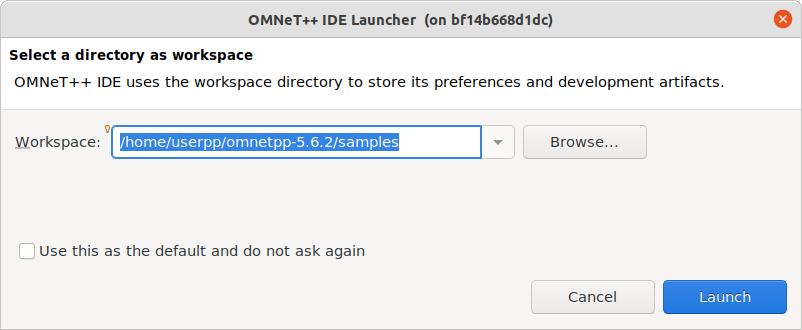
\includegraphics[width=10cm]{workspace}
\end{figure}

Se recomienda usar la ruta /home/userpp/workspace, ya que en general lanzamos
contenedores docker donde esa ruta es un volumen (lo que hacemos desde el
contenedor dentro de ese directorio, se persiste en el host, más allá de la
vida útil del contenedor).

\subsection{Preparando un nuevo proyecto}

Desde el IDE, seleccionar \ui{File $\rightarrow$ New $\rightarrow$ OMNeT++
Project} (fig.~\ref{fig:new_project}). Al aparecer el diálogo, ingresar
\verb!pytictoc! como nombre del proyecto, seleccionar \ui{Empty project} y
luego \ui{Finish}. Un nuevo proyecto aparecerá en el área de proyectos del IDE.

\begin{figure}[h]
\caption{Creación de un nuevo proyecto}
\label{fig:new_project}
\centering
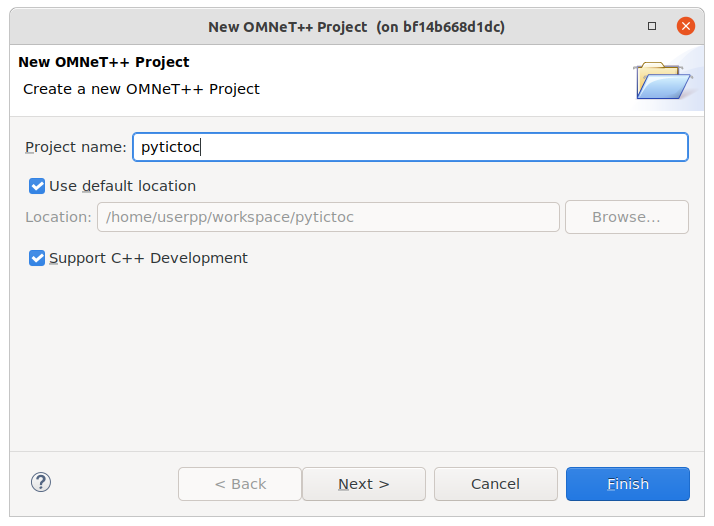
\includegraphics[width=10cm]{new_project}
\end{figure}

\subsection{Agregando un archivo NED}

Hacer click derecho en el proyecto y seleccionar \ui{New $\rightarrow$ Network
Description File (NED)} (fig.~\ref{fig:new_ned}).

\begin{figure}[h]
\caption{Añadir archivo NED}
\label{fig:new_ned}
\centering
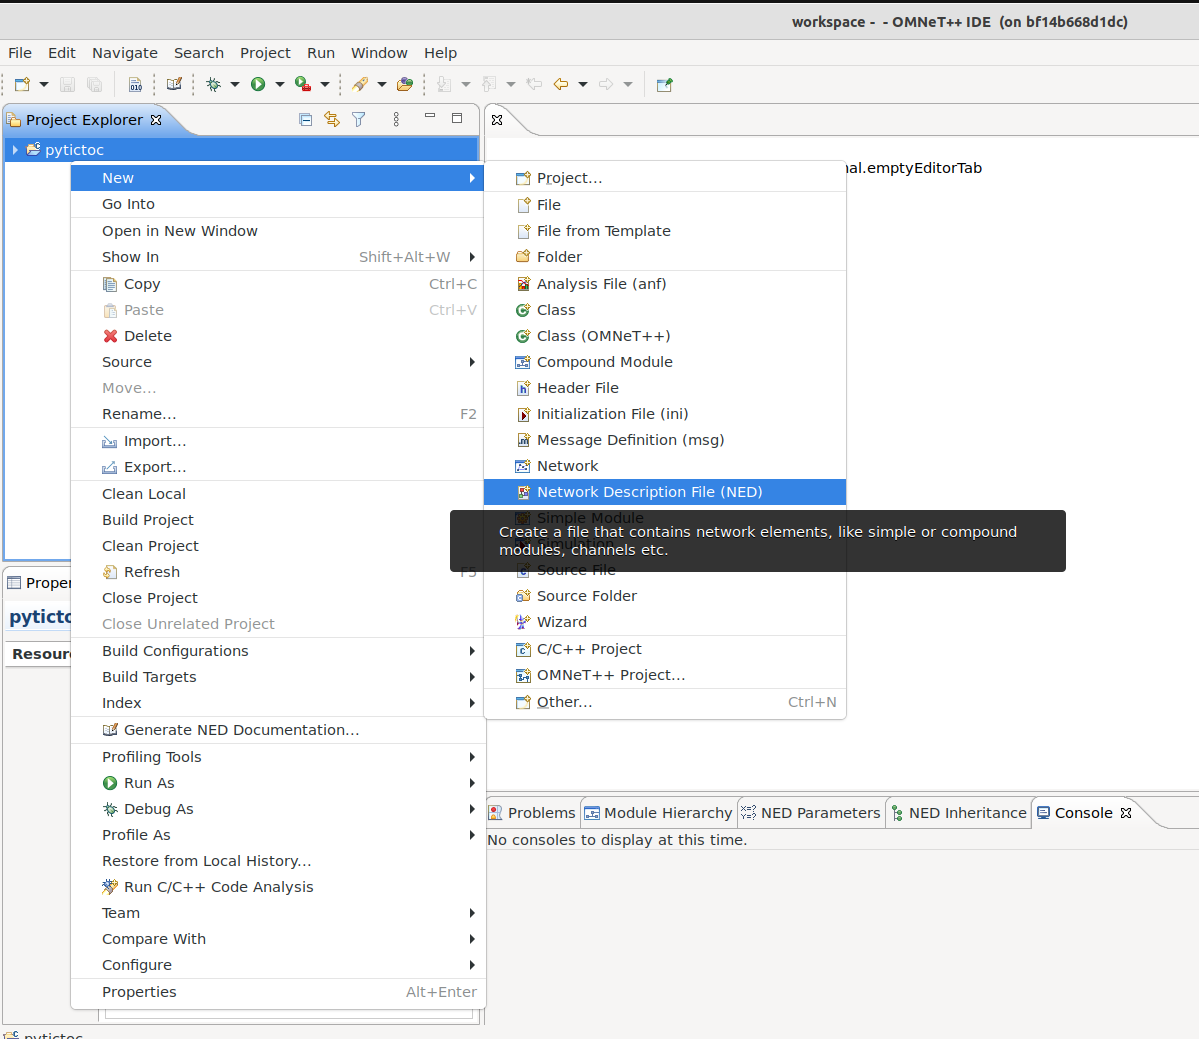
\includegraphics[width=10cm]{add_ned}
\end{figure}

Guardarlo como \verb!pytictoc.ned! con el siguiente contenido:

\inputminted{text}{codelistings/tictoc.ned}

\subsection{Agregando un archivo C++}

Hacer click derecho en el proyecto y seleccionar \ui{New $\rightarrow$ File} y
guardarlo como \verb!txc.cc! con el siguiente contenido:

\inputminted{c++}{codelistings/tictoc.cc}

Dado que el archivo \verb!omnetpy.h! no se encuentra en un directorio conocido
por el IDE, es esperable que se señalen errores en relación a su inclusión o a
\verb!Define_Python_Module!. Para cambiar esto se debe agregar el directorio
\verb!/home/userpp/omnetpy/include! a la lista de directorios escaneados en
busca de archivos de encabezado. En la versión actual del IDE esto se logra en
\ui{Project $\rightarrow$ Properties $\rightarrow$ C/C++ General $\rightarrow$
Path and Symbols} y clickeando el botón \ui{Add}.

\subsection{Agregando un archivo \texttt{makefrag}}

Hacer click derecho en el proyecto, seleccionar \ui{New $\rightarrow$ File} y
guardarlo como \verb!makefrag! con el siguiente contenido:

\begin{minted}[linenos=false]{text}
INCLUDE_PATH += $(shell python3 -m pybind11 --include) -I$(OMNETPY_ROOT)/include
LIBS = -lomnetpy $(shell python3-config --libs | cut -d" " -f1)
LDFLAGS += -L$(OMNETPY_ROOT)/lib
\end{minted}

Estas líneas van a ser incluidas en el archivo \verb!Makefile! autogenerado por
\omnetpp{} para compilar la simulación. Es esencial que se llame
\verb!makefrag!.

\begin{quotation}
\noindent\textbf{Nota importante}: si la versión de Python es 3.8 o mayor,\\
\verb!python3-config --libs!\\
debe reemplazarse por\\
\verb!python3-config --libs --embed!.
\end{quotation}

\subsection{Agregando un archivo Python}

Hacer click derecho en el proyecto, seleccionar \ui{New $\rightarrow$ File} y
guardarlo como \verb!txc.py! con el siguiente contenido:

\inputminted{Python}{codelistings/tictoc.py}

\subsection{Correr la simulación}

En el panel del editor seleccionar el archivo \verb!txc.cc! (la fuente en C++).
Esto es importante para forzar al IDE a ofrecernos la compilación de una
simulación C++ en el siguiente paso.

Seleccionar \ui{Run $\rightarrow$ Run} y elegir \ui{OMNeT++ Simulation} (fig.~\ref{fig:run}).

\begin{figure}[h]
\caption{Correr la simulación}
\label{fig:run}
\centering
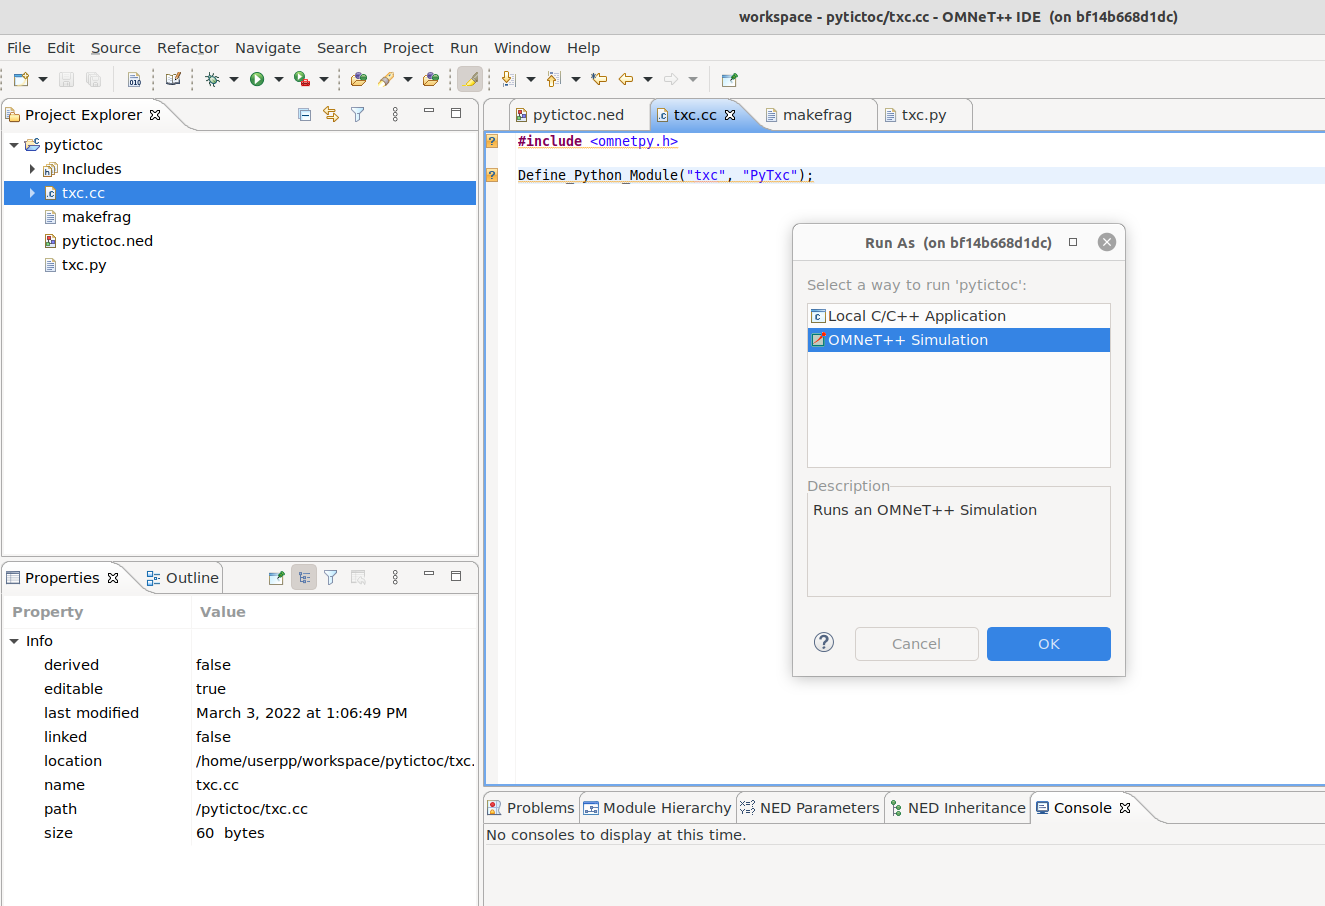
\includegraphics[width=10cm]{run_simulation}
\end{figure}

Luego de la compilación, se lanza automáticamente la ejecución de la
simulación (fig.~\ref{fig:first_run}).


\begin{figure}[h]
\caption{Simulación}
\label{fig:first_run}
\centering
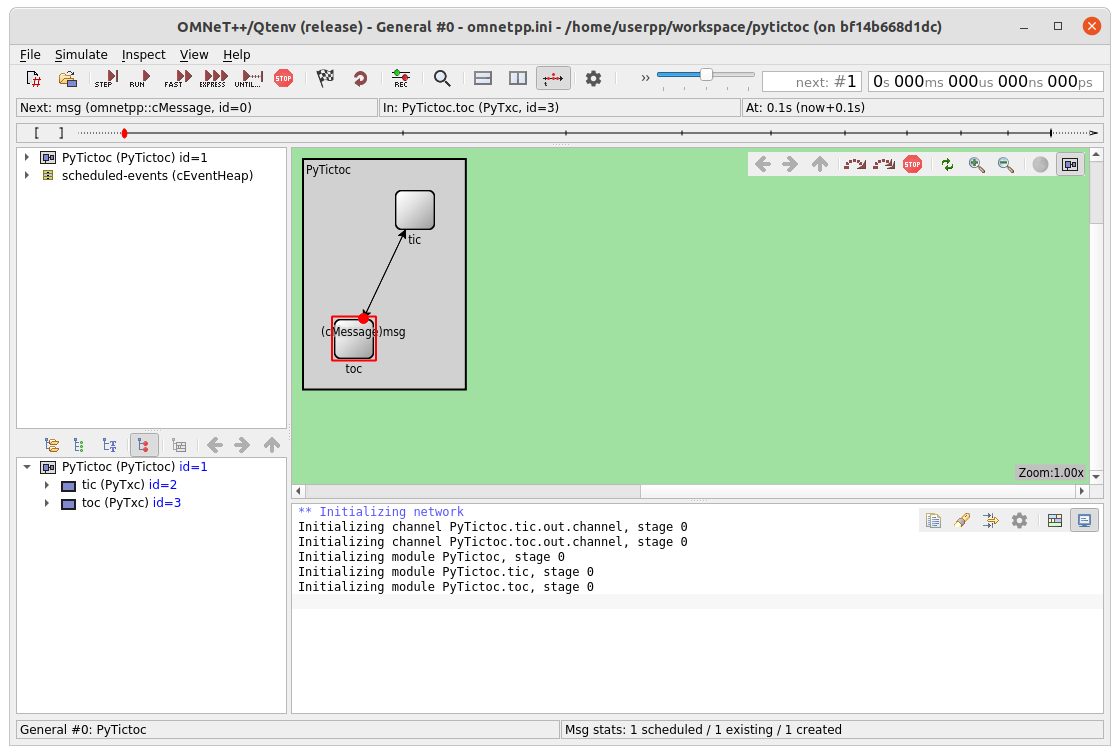
\includegraphics[width=10cm]{first_run}
\end{figure}
